\documentclass[12pt,a4paper]{article}

\usepackage[margin=1in]{geometry}
\usepackage{setspace}
\usepackage{graphicx}
\usepackage{booktabs}
\usepackage{longtable}
\usepackage{array}
\usepackage{hyperref}
\usepackage{xcolor}
\usepackage{listings}
\usepackage{float}
\usepackage{caption}
\usepackage{enumitem}
\usepackage{tabularx}
\usepackage{tikz}
\usetikzlibrary{arrows.meta, positioning}

\onehalfspacing

\hypersetup{
    colorlinks=true,
    linkcolor=blue,
    urlcolor=blue,
    citecolor=blue
}

\lstset{
    basicstyle=\ttfamily\small,
    breaklines=true,
    frame=single,
    columns=fullflexible
}

\title{
    \textbf{Assignment 2: Wireless Protocol Investigation Lab}\\
    \large Track 3: SSID/BSSID Identity and Evil Twin Trust Assumptions
}

\author{
    Aliza Lazar (336392899), Or Bibi (207707613), Meir Shuker (318901527)\\
    Ariel University --- Wireless and Mobile Network Security
}

\date{June 15, 2026}

\begin{document}

\maketitle
\tableofcontents

% =========================================================
\section{Investigative Claim}
% =========================================================

Our investigative claim is:

\begin{quote}
\textit{
We will demonstrate that the SSID is visible in multiple unprotected frame types before any association takes place, that the BSSID is not cryptographically bound to the SSID in WPA2, and that a client will initiate association with a rogue AP presenting a known SSID without detecting the identity mismatch at the protocol level.
}
\end{quote}

In this report, conclusions are phrased as evidence-based observations from our own controlled captures. We do not claim universal behavior for every client, AP, driver, or authentication mode. The analysis is limited to our controlled WPA2-PSK lab setup.

% =========================================================
\section{Evidence Plan}
% =========================================================

The goal of the evidence plan is to define before analysis which packets, fields, parser outputs, and comparisons are needed to evaluate the investigative claim.

\begin{longtable}{|p{4cm}|p{5cm}|p{5cm}|}
\hline
\textbf{Claim Component} & \textbf{Required Evidence} & \textbf{Reason} \\
\hline
SSID is visible before association &
Beacon, Probe Request, Probe Response, and Association Request frames containing \texttt{wlan.ssid} &
Shows that the SSID appears in management frames before key establishment. \\
\hline
Same SSID can be advertised by different BSSIDs &
Modified-condition capture showing AP1 and AP2 advertising the same SSID with different BSSID values &
Shows that the same network name can be presented by more than one AP identity. \\
\hline
Client-selected BSSID can be identified &
Authentication and Association frames sent by the client toward a selected BSSID &
Shows which AP identity the client selected during connection setup. \\
\hline
Key establishment occurs after AP selection &
EAPOL 4-way handshake frames, if present, after Authentication and Association &
Shows that cryptographic key confirmation appears after the client already selected and associated with an AP. \\
\hline
Protocol-level mismatch rejection is not observed in this setup &
No pre-association rejection frame clearly tied to SSID/BSSID identity mismatch &
Supports the claim only within the observed lab setup. \\
\hline
\end{longtable}

\subsection{Frame Types to Capture}

\begin{itemize}
    \item Beacon frames
    \item Probe Request frames
    \item Probe Response frames
    \item Open System Authentication frames
    \item Association Request frames
    \item Association Response frames
    \item EAPOL 4-way handshake frames, if present
\end{itemize}

\subsection{Wireshark Display Filters}

\begin{lstlisting}
Beacon:
wlan.fc.type_subtype == 0x0008

Probe Request:
wlan.fc.type_subtype == 0x0004

Probe Response:
wlan.fc.type_subtype == 0x0005

Authentication:
wlan.fc.type_subtype == 0x000b

Association Request:
wlan.fc.type_subtype == 0x0000

Association Response:
wlan.fc.type_subtype == 0x0001

EAPOL:
eapol
\end{lstlisting}

\subsection{Core Analysis Filters}

\begin{lstlisting}
Full relevant timeline:
(wlan.fc.type == 0 || eapol) &&
(wlan.addr == 32:0a:af:e3:81:b2 ||
 wlan.addr == d6:35:1d:9f:89:fc ||
 wlan.addr == c8:3a:35:c2:e0:b7)

SSID-focused management frames:
wlan.ssid == "Michal_2.4" && wlan.fc.type == 0

BSSID comparison:
wlan.bssid == d6:35:1d:9f:89:fc || wlan.bssid == c8:3a:35:c2:e0:b7
\end{lstlisting}

% =========================================================
\section{Background}
% =========================================================

\subsection{SSID}

The SSID is the human-readable network name displayed to users. In 802.11 networks, the SSID can appear in management frames such as Beacon, Probe Request, Probe Response, and Association Request frames. Per IEEE 802.11, the SSID element is carried in the frame body of these management frames and is not encrypted in a WPA2-PSK network before association completes.

\subsection{BSSID}

The BSSID is the MAC-layer identity of a Basic Service Set. In an infrastructure Wi-Fi network, it is typically the MAC address of the access point radio interface. Two APs may advertise the same SSID while having different BSSIDs.

In our lab:
\begin{itemize}
    \item AP1 SSID: \texttt{Michal\_2.4}
    \item AP1 BSSID: \texttt{d6:35:1d:9f:89:fc}
    \item AP2 SSID: \texttt{Michal\_2.4}
    \item AP2 BSSID: \texttt{c8:3a:35:c2:e0:b7}
\end{itemize}

\subsection{Management Frames}

Management frames are used for discovery, authentication, association, and network capability advertisement. Before key establishment, many management frames are visible to a passive monitor.

In our captures, Beacon frames (subtype \texttt{0x0008}) expose SSID (\texttt{wlan.ssid}), BSSID (\texttt{wlan.bssid}), and the RSN Information Element including AKM suite type, pairwise cipher suite, and PMF capability/requirement bits. Probe Request frames expose the client's requested SSID. Association Request frames expose the SSID and the client's selected RSN parameters. These fields are visible to any passive monitor on the same channel.

\subsection{RSN and WPA2-PSK}

Robust Security Network (RSN) information elements advertise security capabilities such as AKM suites, pairwise ciphers, and PMF capability or requirement bits. In WPA2-PSK, key establishment occurs during the 4-way handshake after authentication and association.

The RSN IE appears in Beacon and Association Request frames. Key fields include AKM suite (\texttt{wlan.rsn.akms.type}, value 2 = PSK), pairwise cipher suite (\texttt{wlan.rsn.pcs.type}), and PMF capability/requirement bits. The 4-way handshake (EAPOL exchange) that follows association derives session keys from the PSK and SSID via PBKDF2, but this binding is not verified at the management frame level before association.

\subsection{Evil Twin Trust Assumption}

An Evil Twin-style scenario involves an AP that presents a known or legitimate-looking SSID. This track investigates the protocol-level identity assumptions involved in this behavior. Our experiment does not attempt credential theft or unauthorized access. It only studies how the client behaves when the same SSID is advertised by different BSSIDs in a controlled lab. Unlike Assignment~1 (active deauthentication attack), Track~3 uses passive observation and a user-initiated reconnect trigger.

% =========================================================
\section{Threat Model}
% =========================================================

\subsection{Assets}

The main asset is correct network identity selection by the client for a saved SSID profile.

\subsection{Attacker Position}

The attacker is modeled as a nearby wireless adversary operating an AP under authorized lab control. This AP is referred to as the rogue-condition AP (AP2). No credential theft is assumed.

\subsection{Attacker Capabilities Within the Lab}

\begin{itemize}
    \item Broadcast the same SSID from a different BSSID.
    \item Influence which AP the client attempts to associate with (same SSID, same WPA2-PSK passphrase).
    \item Observe management frames and AP advertisement behavior in the authorized lab environment.
\end{itemize}

\subsection{Attacker Limitations}

\begin{itemize}
    \item No out-of-scope devices are targeted or analyzed.
    \item No credential cracking is performed.
    \item No deauthentication attack against the legitimate AP was used (not required for Track~3).
    \item No unlawful interference or non-authorized traffic collection is performed.
    \item No real third-party networks are used.
\end{itemize}

\subsection{Security Question Tested}

The security question tested is whether, in our WPA2-PSK lab setup, the client's pre-association network selection can be explained by visible SSID/profile matching and selected BSSID behavior, while SSID information appears in unprotected management frames.

% =========================================================
\section{Lab Setup}
% =========================================================

\subsection{Topology}

\begin{figure}[H]
\centering
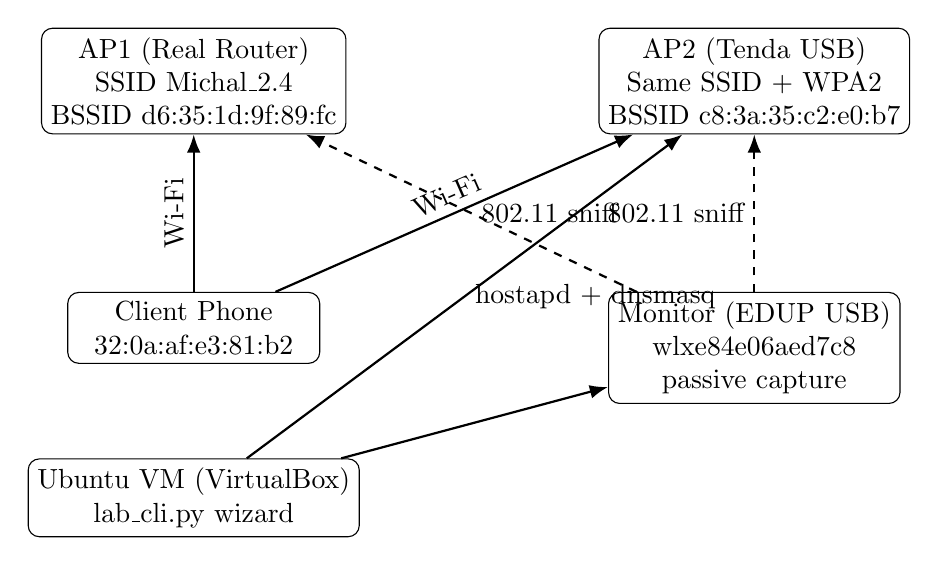
\begin{tikzpicture}[
    node distance=1.6cm,
    box/.style={draw, rounded corners, align=center, minimum width=3.2cm, minimum height=0.9cm},
    arrow/.style={-Latex, thick}
]
\node[box] (ap1) {AP1 (Real Router)\\SSID Michal\_2.4\\BSSID d6:35:1d:9f:89:fc};
\node[box, right=3.2cm of ap1] (ap2) {AP2 (Tenda USB)\\Same SSID + WPA2\\BSSID c8:3a:35:c2:e0:b7};
\node[box, below=2cm of ap1] (client) {Client Phone\\32:0a:af:e3:81:b2};
\node[box, below=2cm of ap2] (mon) {Monitor (EDUP USB)\\wlxe84e06aed7c8\\passive capture};
\node[box, below=1.2cm of client] (vm) {Ubuntu VM (VirtualBox)\\lab\_cli.py wizard};

\draw[arrow] (client) -- node[above, sloped] {Wi-Fi} (ap1);
\draw[arrow] (client) -- node[above, sloped] {Wi-Fi} (ap2);
\draw[dashed, arrow] (mon) -- node[right] {802.11 sniff} (ap1);
\draw[dashed, arrow] (mon) -- node[left] {802.11 sniff} (ap2);
\draw[arrow] (vm) -- (mon);
\draw[arrow] (vm) -- node[right] {hostapd + dnsmasq} (ap2);
\end{tikzpicture}
\caption{Lab topology. AP1 is the legitimate home router. AP2 is a controlled rogue-condition AP on a Tenda USB adapter. The EDUP adapter captures management and EAPOL frames in monitor mode.}
\end{figure}

\subsection{Devices}

\begin{table}[H]
\centering
\begin{tabular}{|p{3cm}|p{4cm}|p{6cm}|}
\hline
\textbf{Device} & \textbf{Role} & \textbf{Details} \\
\hline
AP1 & Baseline AP & Home router, SSID \texttt{Michal\_2.4}, BSSID \texttt{d6:35:1d:9f:89:fc}, channel 12, WPA2-PSK \\
\hline
AP2 & Rogue-condition AP & Tenda USB (Ralink \texttt{148f:3070}), interface \texttt{wlxc83a35c2e0b7}, BSSID \texttt{c8:3a:35:c2:e0:b7}, hostapd + dnsmasq DHCP \\
\hline
Client & Wi-Fi client & Smartphone, MAC \texttt{32:0a:af:e3:81:b2}, saved WPA2 profile for \texttt{Michal\_2.4} \\
\hline
Monitor station & Passive capture & Ubuntu 24.04 VM, EDUP USB (MediaTek \texttt{0e8d:7961}), interface \texttt{wlxe84e06aed7c8}, MAC \texttt{e8:4e:06:ae:d7:c8} \\
\hline
\end{tabular}
\caption{Lab devices and roles.}
\end{table}

\subsection{Network Configuration}

\begin{table}[H]
\centering
\begin{tabular}{|p{5cm}|p{8cm}|}
\hline
\textbf{Parameter} & \textbf{Value} \\
\hline
Target SSID & \texttt{Michal\_2.4} \\
\hline
Security mode & WPA2-PSK (CCMP) \\
\hline
Password / PSK & Omitted from report (configured identically on AP1 and AP2) \\
\hline
AP1 BSSID & \texttt{d6:35:1d:9f:89:fc} \\
\hline
AP2 BSSID & \texttt{c8:3a:35:c2:e0:b7} \\
\hline
Channel & 12 \\
\hline
Band & 2.4 GHz \\
\hline
Physical placement & AP1 (router), AP2 (Tenda USB), monitor (EDUP USB), and client phone in the same room; VM on same host \\
\hline
\end{tabular}
\caption{Network configuration.}
\end{table}

\subsection{Capture Setup Commands}

Captures were collected using the project wizard (\texttt{sudo .venv/bin/python lab\_cli.py}), which automates monitor mode, 25-second timed captures, filtering, and parsing. Equivalent manual commands:

\begin{lstlisting}
sudo ip link set wlxe84e06aed7c8 down
sudo iw dev wlxe84e06aed7c8 set type monitor
sudo ip link set wlxe84e06aed7c8 up
sudo iw dev wlxe84e06aed7c8 set channel 12

sudo timeout 25 tcpdump -i wlxe84e06aed7c8 \
  -w captures/track3_same_ssid_baseline_ap1_only.pcapng

sudo timeout 25 tcpdump -i wlxe84e06aed7c8 \
  -w captures/track3_same_ssid_modified_ap1_ap2.pcapng
\end{lstlisting}

Filtered evidence captures:

\begin{lstlisting}
tshark -r captures/track3_same_ssid_baseline_ap1_only.pcapng \
  -Y "(wlan.fc.type==0 || eapol) && (wlan.addr==32:0a:af:e3:81:b2 || wlan.addr==d6:35:1d:9f:89:fc)" \
  -w captures/track3_filtered_baseline_authorized_only.pcapng

tshark -r captures/track3_same_ssid_modified_ap1_ap2.pcapng \
  -Y "(wlan.fc.type==0 || eapol) && (wlan.addr==32:0a:af:e3:81:b2 || wlan.addr==d6:35:1d:9f:89:fc || wlan.addr==c8:3a:35:c2:e0:b7)" \
  -w captures/track3_filtered_modified_authorized_only.pcapng
\end{lstlisting}

% =========================================================
\section{Experiment Design}
% =========================================================

\subsection{Baseline Condition}

In the baseline condition, AP1 is active and AP2 is disabled. The client triggers a reconnect (Wi-Fi off/on) during a 25-second capture window while AP2 is off.

\begin{itemize}
    \item AP1 active: Yes
    \item AP2 active: No
    \item SSID: \texttt{Michal\_2.4}
    \item Expected observation: The client reconnects toward AP1.
    \item Capture file: \texttt{track3\_same\_ssid\_baseline\_ap1\_only.pcapng} (116\,165 bytes)
\end{itemize}

\subsection{Modified Condition}

In the modified condition, AP1 and AP2 are both active. Both APs advertise the same SSID and use the same WPA2-PSK credentials, but they have different BSSIDs. AP2 also runs dnsmasq (DHCP \texttt{10.0.0.1}) so the client can complete L2/L3 setup. The client performed two manual reconnect cycles during the 25-second capture.

\begin{itemize}
    \item AP1 active: Yes
    \item AP2 active: Yes (hostapd + dnsmasq)
    \item Same SSID: Yes
    \item Different BSSID: Yes
    \item Expected observation: The client may select either BSSID; we observe which BSSID receives Auth/Assoc/EAPOL.
    \item Capture file: \texttt{track3\_same\_ssid\_modified\_ap1\_ap2.pcapng} (252\,327 bytes)
\end{itemize}

\subsection{Controlled Variable}

The intentional changed variable is AP identity availability (the BSSID set available for the same SSID). The SSID, security mode, credentials, client MAC, monitor adapter, channel, and capture workflow remained fixed.

% =========================================================
\section{Packet Evidence}
% =========================================================

\subsection{Capture Files}

\begin{table}[H]
\centering
\begin{tabular}{|p{6cm}|p{7cm}|}
\hline
\textbf{File Name} & \textbf{Purpose / Size} \\
\hline
\texttt{track3\_same\_ssid\_baseline\_ap1\_only.pcapng} & Raw baseline (116 KB) \\
\hline
\texttt{track3\_same\_ssid\_modified\_ap1\_ap2.pcapng} & Raw modified (252 KB) \\
\hline
\texttt{track3\_filtered\_baseline\_authorized\_only.pcapng} & Filtered baseline (35 KB) \\
\hline
\texttt{track3\_filtered\_modified\_authorized\_only.pcapng} & Filtered modified (84 KB) \\
\hline
\end{tabular}
\caption{Capture files used in the investigation.}
\end{table}

\subsection{Annotated Packet Table --- Baseline}

Frames refer to \texttt{track3\_filtered\_baseline\_authorized\_only.pcapng} unless noted.

\begin{table}[H]
\centering
\scriptsize
\renewcommand{\arraystretch}{1.3}
\begin{tabularx}{\textwidth}{|c|c|c|c|c|X|}
\hline
\textbf{Fr.} & \textbf{Subtype} & \textbf{Tx} & \textbf{Rx} & \textbf{BSSID} & \textbf{Interpretation} \\
\hline
1 & 0x0008 Beacon & d6:35:1d:9f:89:fc & broadcast & d6:35:1d:9f:89:fc & AP1 advertises \texttt{Michal\_2.4} in clear text. \\
\hline
16 & 0x0004 Probe Req. & 32:0a:af:e3:81:b2 & broadcast & --- & Client probes for \texttt{Michal\_2.4} before association. \\
\hline
17 & EAPOL (0x0028) & 32:0a:af:e3:81:b2 & d6:35:1d:9f:89:fc & d6:35:1d:9f:89:fc & WPA2 key exchange with AP1 (EAPOL message 2 observed). \\
\hline
19--24 & 0x000d Data & client $\leftrightarrow$ AP1 & d6:35:1d:9f:89:fc & Post-association traffic with AP1. \\
\hline
\end{tabularx}
\caption{Baseline packet evidence (AP2 off). Full Auth/Assoc may be abbreviated when PMKSA cache is used; EAPOL to AP1 confirms reconnect toward the legitimate BSSID.}
\end{table}

\begin{figure}[H]
\centering
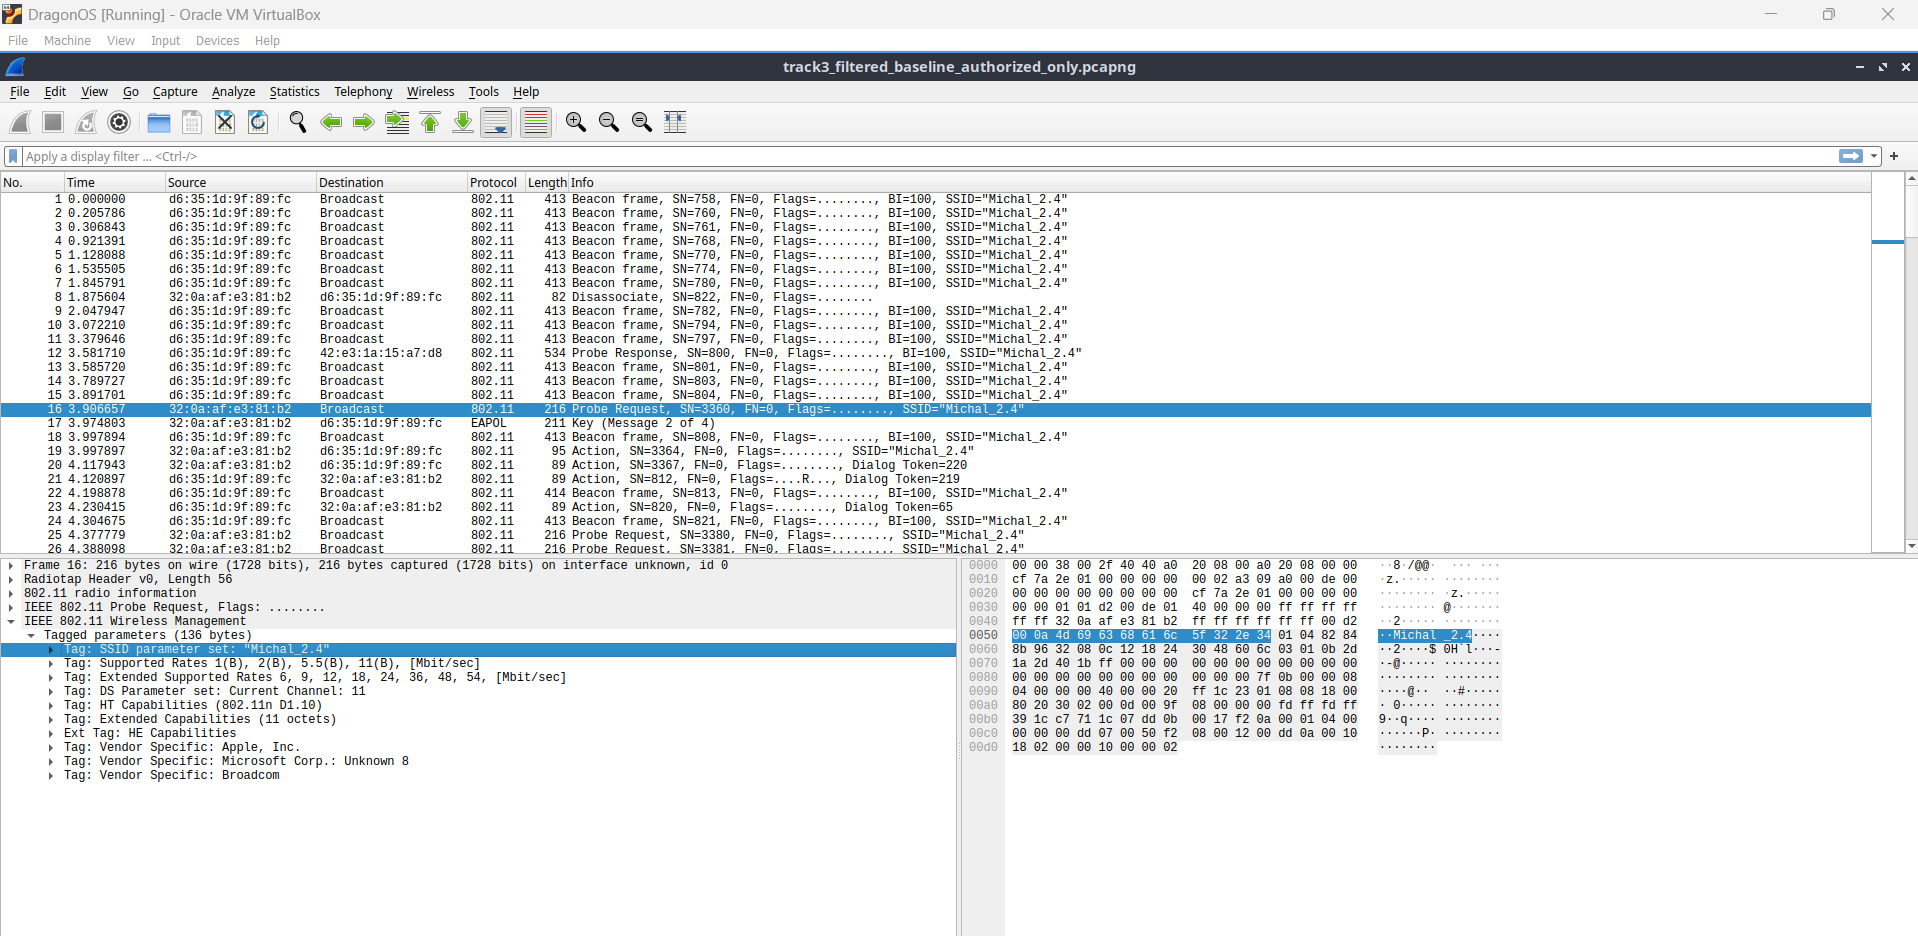
\includegraphics[width=0.95\textwidth]{figures/baseline_probe.png}
\caption{Baseline Wireshark evidence: Probe Request (frame 16) for \texttt{Michal\_2.4} from client \texttt{32:0a:af:e3:81:b2}.}
\end{figure}

\begin{figure}[H]
\centering
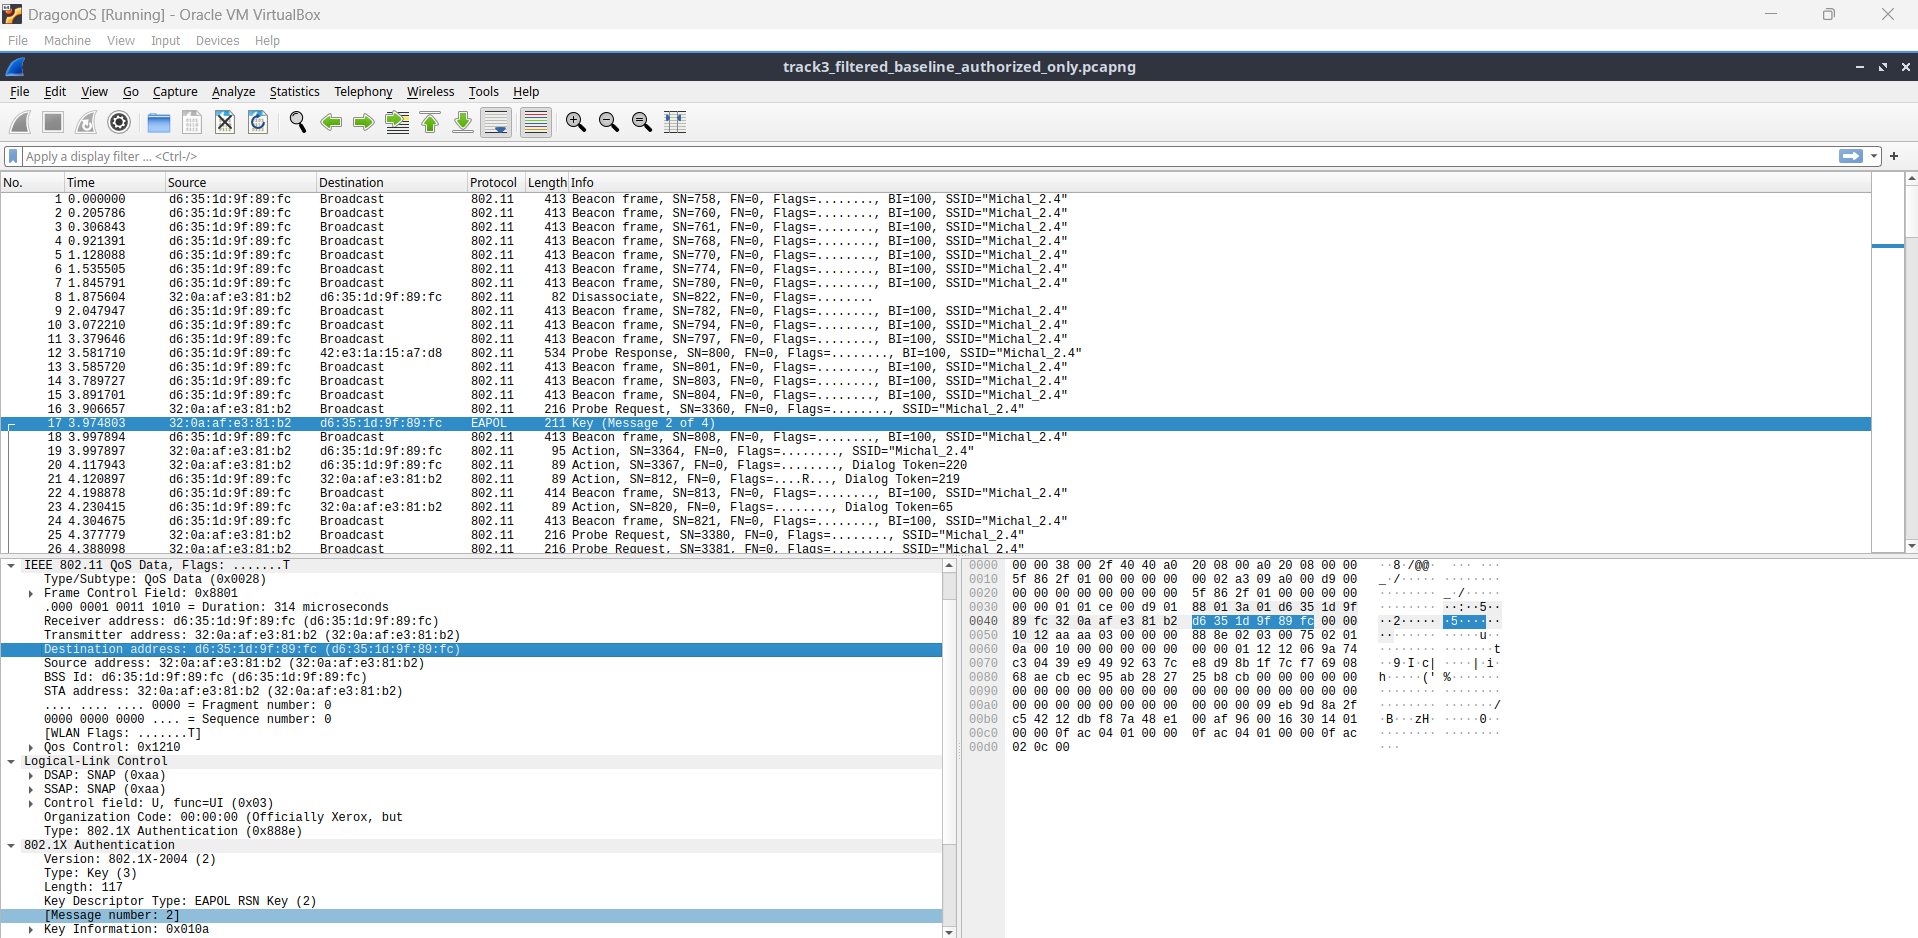
\includegraphics[width=0.95\textwidth]{figures/baseline_eapol_ap1.png}
\caption{Baseline Wireshark evidence: EAPOL message 2 (frame 17) sent toward AP1 (\texttt{d6:35:1d:9f:89:fc}), confirming key-establishment traffic with the legitimate BSSID.}
\end{figure}

\subsection{Annotated Packet Table --- Modified}

Frames refer to \texttt{track3\_filtered\_modified\_authorized\_only.pcapng}. Raw modified capture: 241 Beacons from AP2 and 45 from AP1 with \texttt{wlan.ssid == "Michal\_2.4"}.

\begin{table}[H]
\centering
\scriptsize
\renewcommand{\arraystretch}{1.3}
\begin{tabularx}{\textwidth}{|c|c|c|c|c|X|}
\hline
\textbf{Fr.} & \textbf{Subtype} & \textbf{Tx} & \textbf{Rx} & \textbf{BSSID} & \textbf{Interpretation} \\
\hline
4, 89 & 0x0008 Beacon & AP1 / AP2 & broadcast & both & Same SSID from two different BSSIDs. \\
\hline
68--70 & 0x000b Auth & client $\leftrightarrow$ AP2 & c8:3a:35:c2:e0:b7 & Open System Authentication with AP2 (cycle 1). \\
\hline
71--72 & 0x0000 Assoc Req. & 32:0a:af:e3:81:b2 & AP2 & c8:3a:35:c2:e0:b7 & Client requests association with AP2. \\
\hline
74 & 0x0001 Assoc Resp. & AP2 & client & c8:3a:35:c2:e0:b7 & AP2 accepts association. \\
\hline
75--78 & EAPOL & client $\leftrightarrow$ AP2 & c8:3a:35:c2:e0:b7 & Full 4-way handshake with AP2 (cycle 1). \\
\hline
193--202 & Auth/Assoc/EAPOL & client $\leftrightarrow$ AP2 & c8:3a:35:c2:e0:b7 & Second reconnect cycle (user toggled Wi-Fi twice). \\
\hline
\end{tabularx}
\caption{Modified packet evidence (AP1 + AP2 on). Client selected AP2, not AP1, for both connection cycles.}
\end{table}

\begin{figure}[H]
\centering
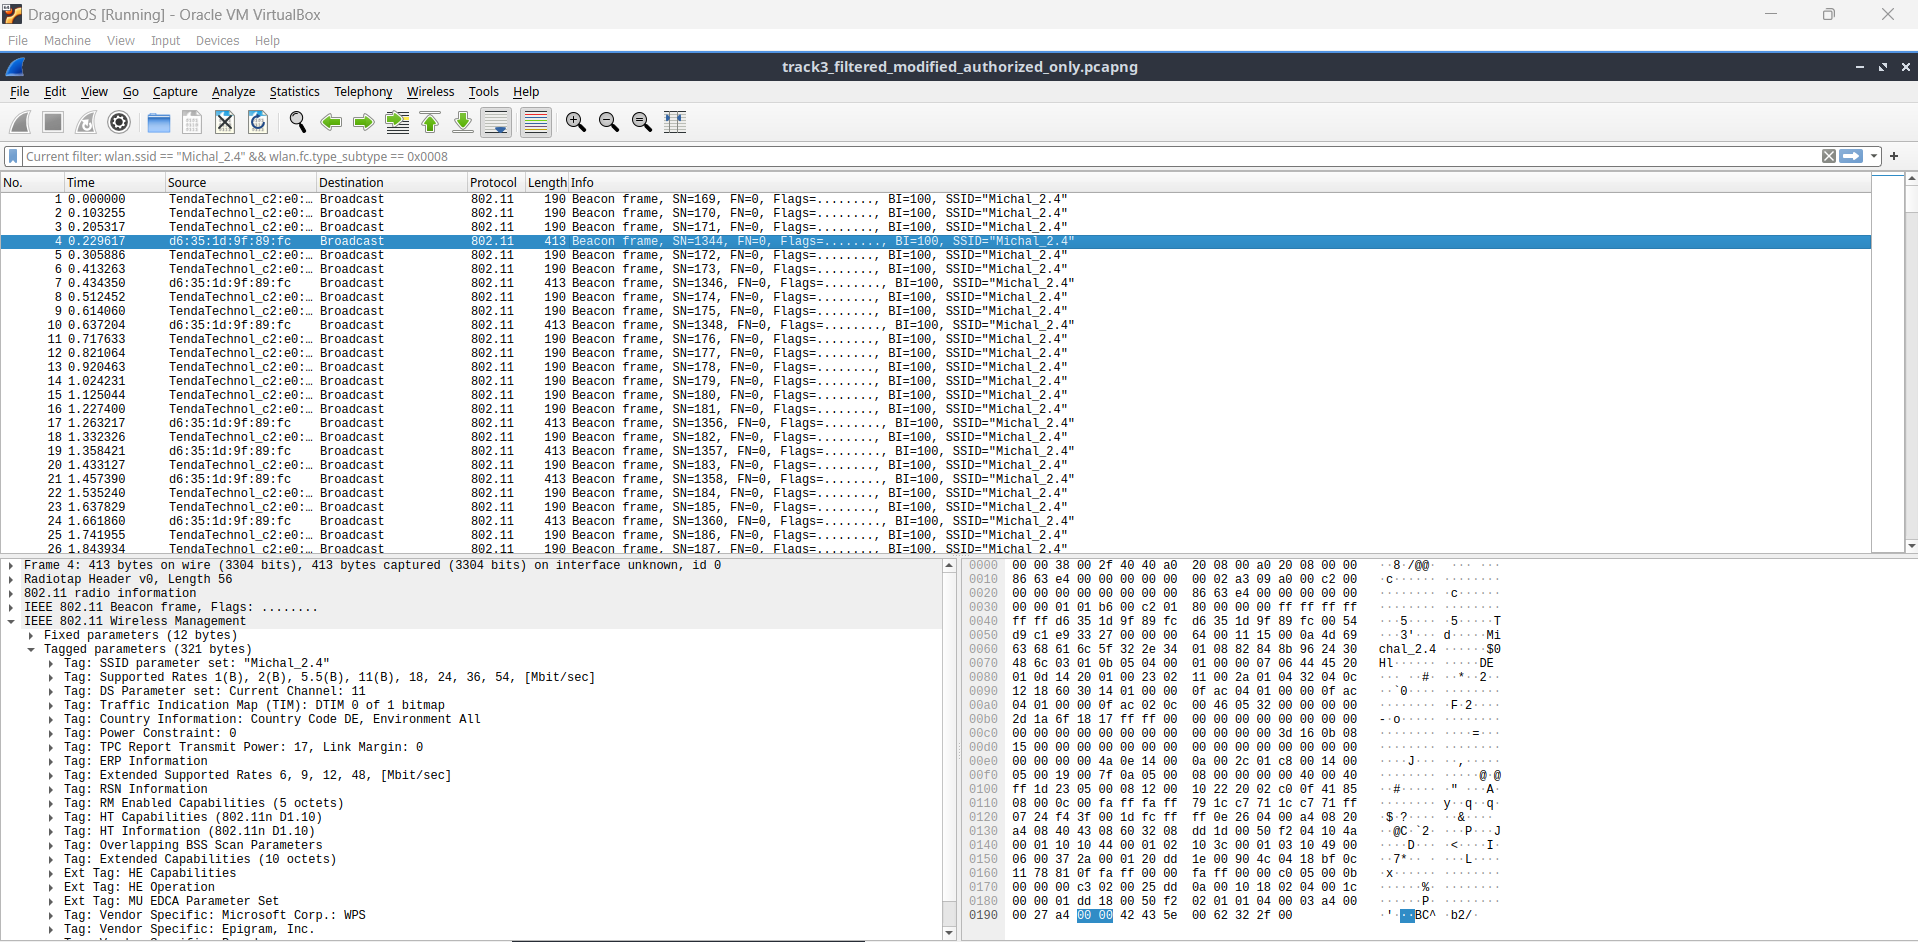
\includegraphics[width=0.95\textwidth]{figures/modified_dual_beacon.png}
\caption{Modified Wireshark evidence: Beacon frames for \texttt{Michal\_2.4} from AP1 (\texttt{d6:35:1d:9f:89:fc}, frame 4) and AP2 (\texttt{c8:3a:35:c2:e0:b7}).}
\end{figure}

\begin{figure}[H]
\centering
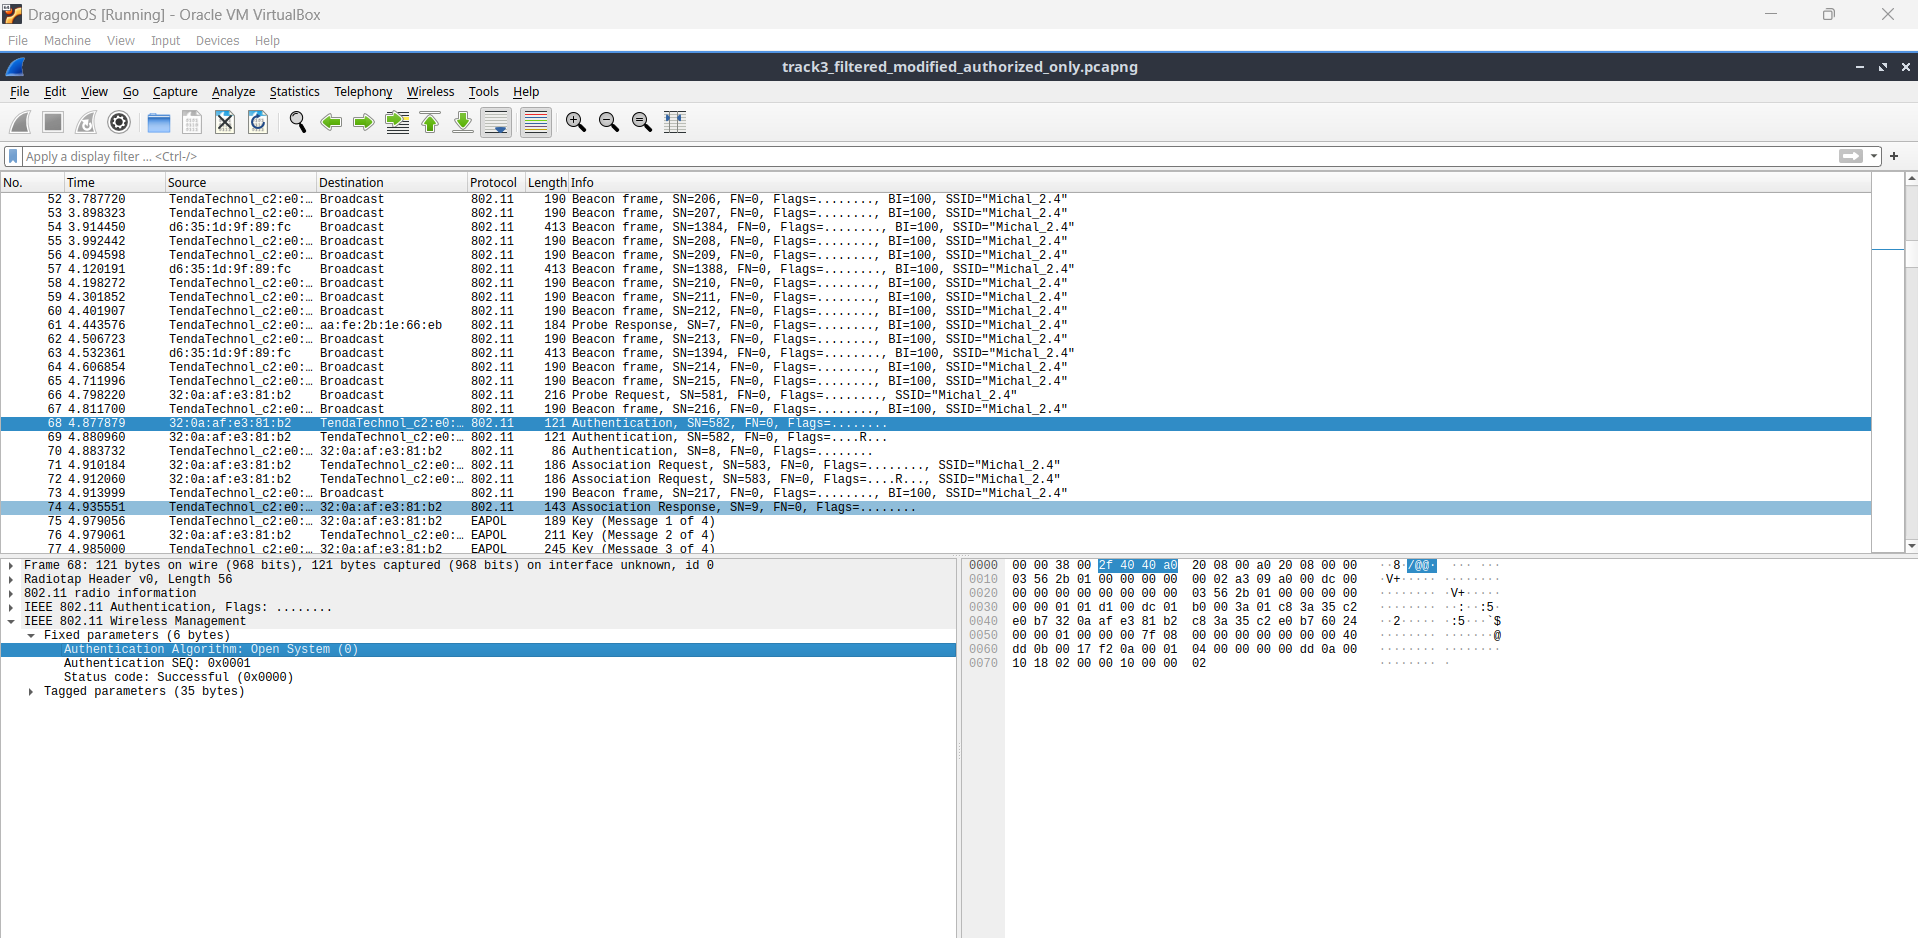
\includegraphics[width=0.95\textwidth]{figures/modified_auth_request.png}
\caption{Modified Wireshark evidence: Open System Authentication request (frame 68) from client to AP2.}
\end{figure}

\begin{figure}[H]
\centering
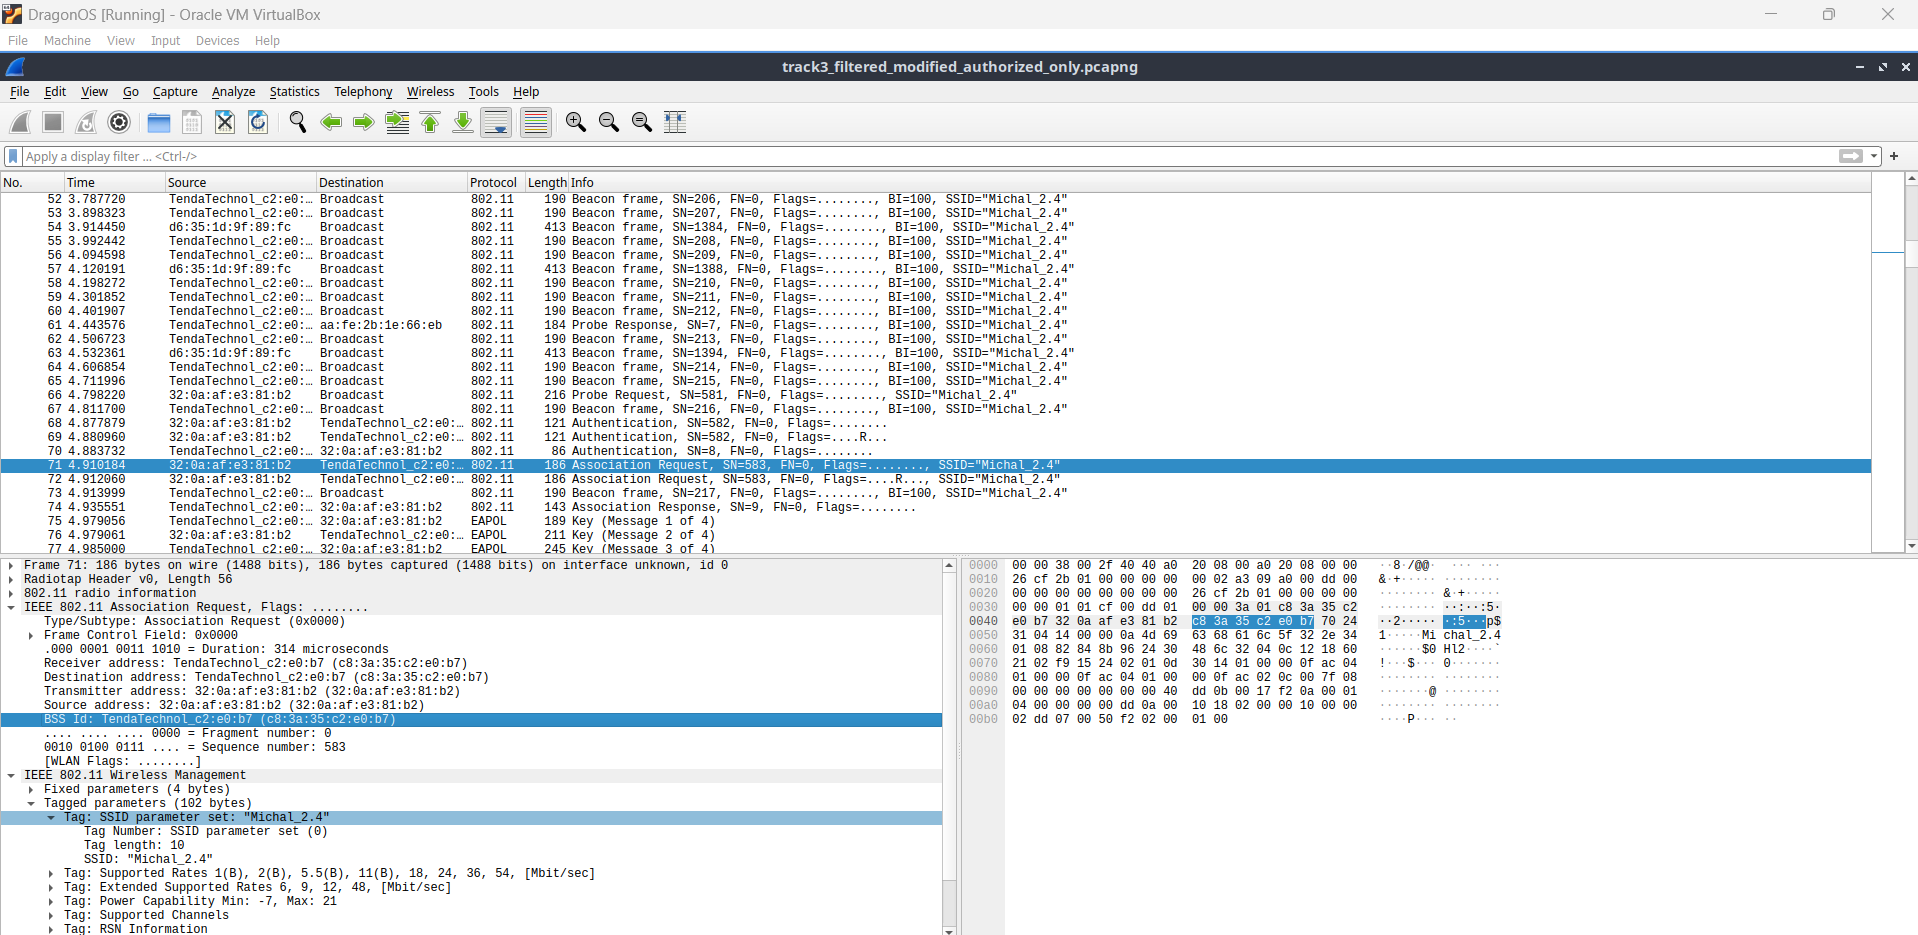
\includegraphics[width=0.95\textwidth]{figures/modified_assoc_request.png}
\caption{Modified Wireshark evidence: Association Request (frame 71) for \texttt{Michal\_2.4} toward AP2 BSSID \texttt{c8:3a:35:c2:e0:b7}.}
\end{figure}

\begin{figure}[H]
\centering
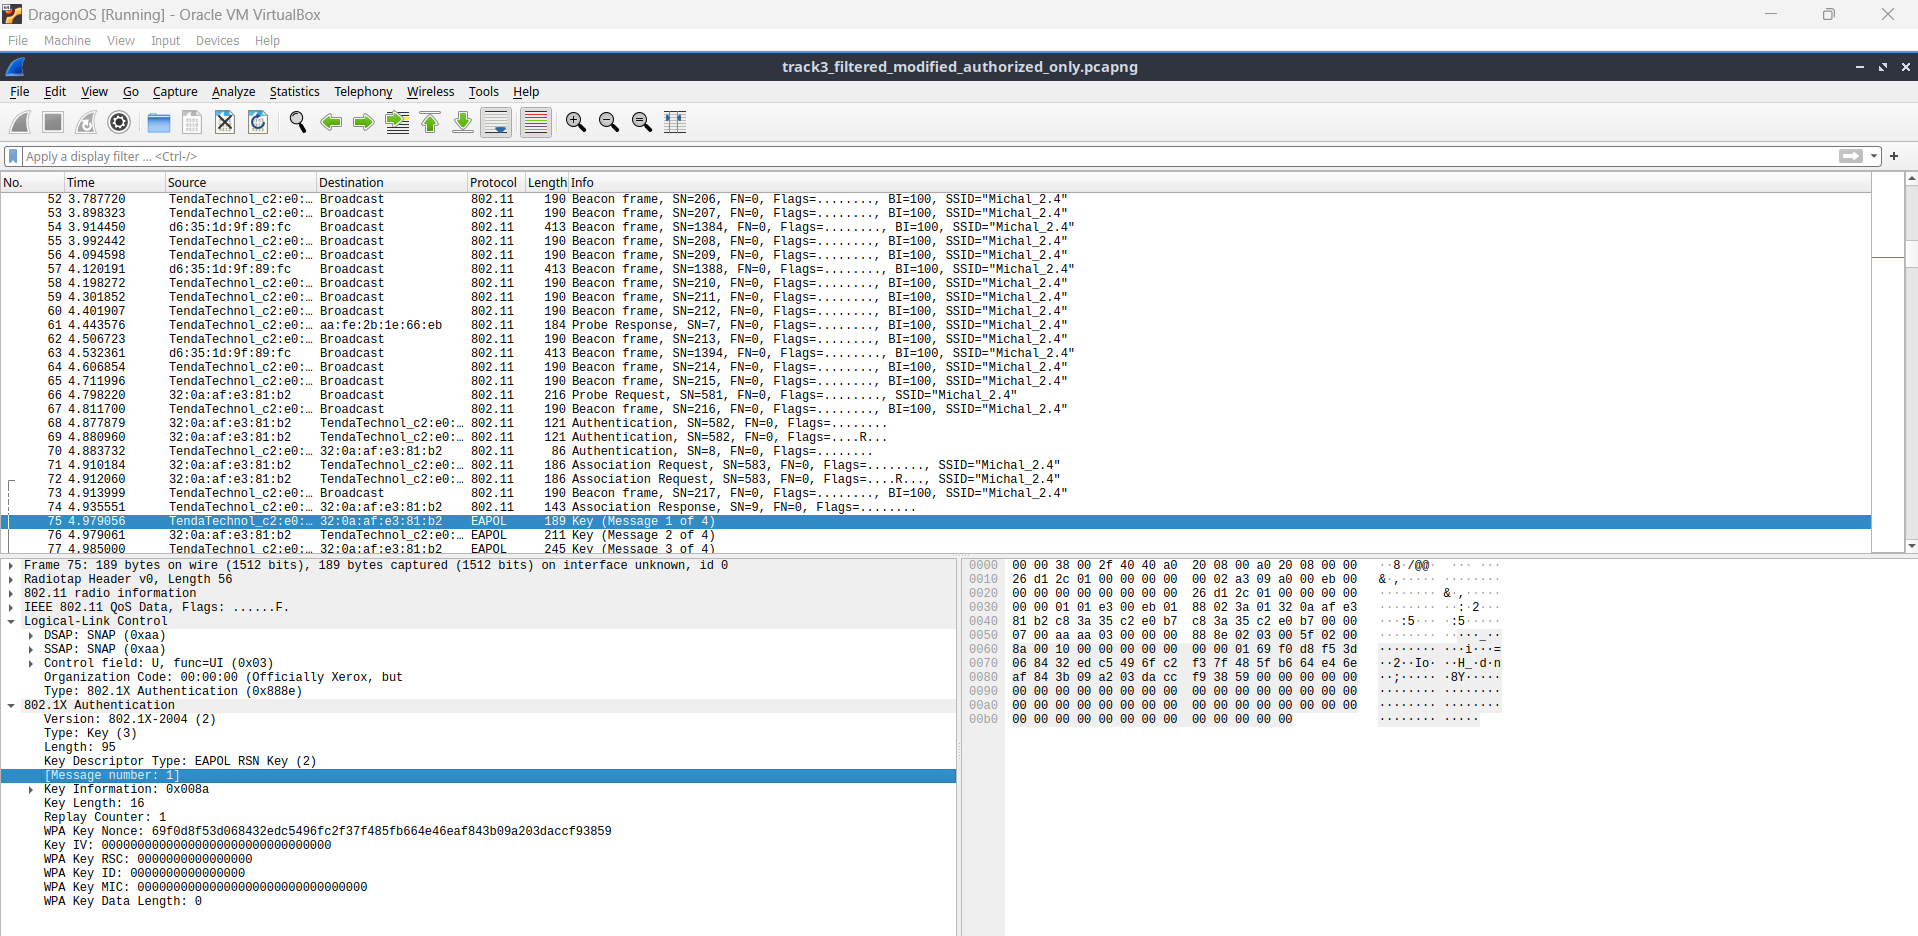
\includegraphics[width=0.95\textwidth]{figures/modified_eapol_msg1.png}
\caption{Modified Wireshark evidence: EAPOL 4-way handshake message 1 (frame 75) with AP2.}
\end{figure}

\subsection{TShark Excerpts}

Example extraction command:

\begin{lstlisting}
tshark -r captures/track3_filtered_modified_authorized_only.pcapng \
  -Y "wlan.addr==32:0a:af:e3:81:b2 && (eapol || wlan.fc.type_subtype==0x0b || wlan.fc.type_subtype==0x0)" \
  -T fields -e frame.number -e wlan.bssid -e wlan.fc.type_subtype
\end{lstlisting}

Observed output (abbreviated):
\begin{lstlisting}
68  c8:3a:35:c2:e0:b7  0x000b
71  c8:3a:35:c2:e0:b7  0x0000
74  c8:3a:35:c2:e0:b7  0x0001
75  c8:3a:35:c2:e0:b7  0x0028
193 c8:3a:35:c2:e0:b7  0x000b
195 c8:3a:35:c2:e0:b7  0x0000
\end{lstlisting}

Hostapd log (\texttt{hostapd\_ap2.log}) corroborates two complete handshakes:
\begin{lstlisting}
AP-STA-CONNECTED 32:0a:af:e3:81:b2
EAPOL-4WAY-HS-COMPLETED 32:0a:af:e3:81:b2
AP-STA-DISCONNECTED 32:0a:af:e3:81:b2
AP-STA-CONNECTED 32:0a:af:e3:81:b2
EAPOL-4WAY-HS-COMPLETED 32:0a:af:e3:81:b2
\end{lstlisting}

% =========================================================
\section{Parser / Analysis Output}
% =========================================================

\subsection{Parser Overview}

We implemented \texttt{parser/ssid\_track3\_parser.py} in Python~3 using PyShark for PCAP/PCAPNG parsing. The wizard (\texttt{lab\_cli.py}) runs the parser automatically in step~10.

\subsection{Parser Command}

\begin{lstlisting}
.venv/bin/python parser/ssid_track3_parser.py \
  --pcap captures/track3_filtered_baseline_authorized_only.pcapng \
  --pcap captures/track3_filtered_modified_authorized_only.pcapng \
  --output-dir outputs \
  --target-ssid "Michal_2.4" \
  --ap1-bssid d6:35:1d:9f:89:fc \
  --ap2-bssid c8:3a:35:c2:e0:b7
\end{lstlisting}

\subsection{Parser Output Summary}

\begin{table}[H]
\centering
\begin{tabular}{|p{5cm}|p{8cm}|}
\hline
\textbf{Output Item} & \textbf{Result} \\
\hline
Total parsed records & 414 \\
\hline
Discovery-phase frames & 385 \\
\hline
Auth/Assoc frames & 10 \\
\hline
EAPOL (key exchange) frames & 9 \\
\hline
AP BSSIDs advertising target SSID (TShark on raw modified) & 2 (\texttt{d6:35:1d:...}, \texttt{c8:3a:35:...}) \\
\hline
Client-selected BSSID in baseline & \texttt{d6:35:1d:9f:89:fc} (EAPOL frame 17) \\
\hline
Client-selected BSSID in modified & \texttt{c8:3a:35:c2:e0:b7} (frames 68--78, 193--202) \\
\hline
EAPOL handshake observed & Yes \\
\hline
\end{tabular}
\caption{Parser and manual verification summary.}
\end{table}

\textbf{Note on \texttt{claim\_summary.json}:} The automated flags \texttt{ssid\_visible\_pre\_assoc=false} and \texttt{same\_ssid\_advertised\_by\_multiple\_bssids=false} are false negatives: PyShark often leaves the \texttt{ssid} CSV field empty for Beacon frames even when \texttt{wlan.ssid} is present in the PCAP (verified with TShark). We therefore cite frame-level PCAP evidence for SSID visibility and dual-BSSID advertisement.

% =========================================================
\section{Protocol Sequence / State-Machine Diagram}
% =========================================================

\begin{figure}[H]
\centering
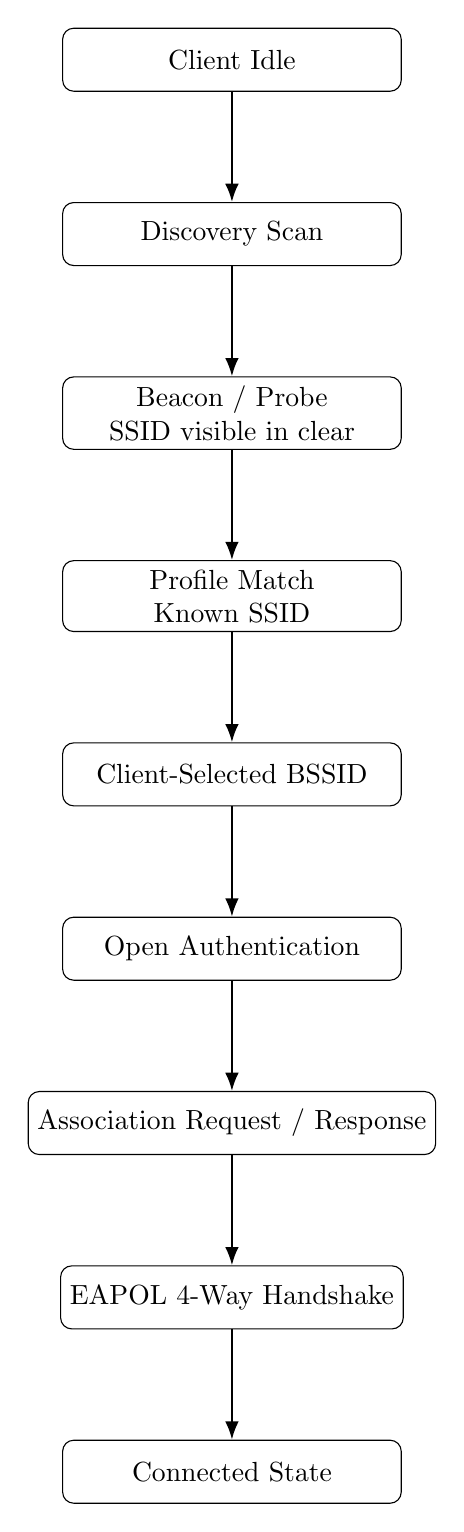
\begin{tikzpicture}[
    node distance=1.4cm,
    every node/.style={draw, rounded corners, align=center, minimum width=4.3cm, minimum height=0.8cm},
    arrow/.style={-Latex, thick}
]
\node (idle) {Client Idle};
\node (scan) [below=of idle] {Discovery Scan};
\node (beacon) [below=of scan] {Beacon / Probe\\SSID visible in clear};
\node (profile) [below=of beacon] {Profile Match\\Known SSID};
\node (bssid) [below=of profile] {Client-Selected BSSID};
\node (auth) [below=of bssid] {Open Authentication};
\node (assoc) [below=of auth] {Association Request / Response};
\node (eapol) [below=of assoc] {EAPOL 4-Way Handshake};
\node (connected) [below=of eapol] {Connected State};

\draw[arrow] (idle) -- (scan);
\draw[arrow] (scan) -- (beacon);
\draw[arrow] (beacon) -- (profile);
\draw[arrow] (profile) -- (bssid);
\draw[arrow] (bssid) -- (auth);
\draw[arrow] (auth) -- (assoc);
\draw[arrow] (assoc) -- (eapol);
\draw[arrow] (eapol) -- (connected);
\end{tikzpicture}
\caption{Protocol sequence for same-SSID/different-BSSID investigation.}
\end{figure}

\textbf{Observed frame mapping:}
\begin{itemize}
    \item Baseline: Probe (fr.\ 16) $\rightarrow$ EAPOL to AP1 (fr.\ 17) $\rightarrow$ data to AP1.
    \item Modified cycle~1: Beacon AP1+AP2 $\rightarrow$ Auth (68--70) $\rightarrow$ Assoc (71--74) $\rightarrow$ EAPOL (75--78) with AP2.
    \item Modified cycle~2: Auth (193--194) $\rightarrow$ Assoc (195, 197) $\rightarrow$ EAPOL (198--202) with AP2.
\end{itemize}

\section{Claim-to-Evidence Table}

\begin{table}[H]
\centering
\scriptsize
\renewcommand{\arraystretch}{1.35}
\begin{tabularx}{\textwidth}{|p{3.2cm}|X|X|X|}
\hline
\textbf{Claim} & \textbf{Evidence} & \textbf{Explanation} & \textbf{Weakening Result} \\
\hline

SSID in unprotected pre-association traffic &
Baseline fr.\ 1 (Beacon), fr.\ 16 (Probe Request); modified fr.\ 4, 89 (Beacons) &
SSID \texttt{Michal\_2.4} appears in management frames before EAPOL &
No SSID in pre-association frames \\
\hline

Same SSID, multiple BSSIDs &
Modified raw: Beacons with \texttt{wlan.ssid==Michal\_2.4} from \texttt{d6:35:1d:9f:89:fc} and \texttt{c8:3a:35:c2:e0:b7} &
Two AP identities broadcast the same network name &
Only one BSSID seen for target SSID \\
\hline

Client-selected BSSID identifiable &
Baseline EAPOL fr.\ 17 $\rightarrow$ AP1; modified Auth/Assoc fr.\ 68--74, 193--197 $\rightarrow$ AP2 &
Authentication and association target a specific BSSID &
Ambiguous or missing Auth/Assoc \\
\hline

Auth/Assoc before EAPOL &
Modified: fr.\ 68--74 then 75--78; baseline: fr.\ 17 EAPOL after probe &
AP selection precedes key-establishment evidence &
EAPOL before Auth/Assoc \\
\hline

No protocol-level BSSID mismatch rejection &
Client completes Auth/Assoc/EAPOL with AP2 despite different BSSID from saved AP1 profile &
No rejection tied to BSSID change alone in our setup &
Explicit reject due to BSSID mismatch \\
\hline
\end{tabularx}
\caption{Claim-to-evidence mapping.}
\end{table}

% =========================================================
\section{Security Analysis}
% =========================================================

\subsection{Where the SSID Appears in the Trace}

\begin{itemize}
    \item Beacon frames: AP1 fr.\ 1; AP1 and AP2 fr.\ 4, 89 (modified).
    \item Probe Request frames: client fr.\ 16, 25 (baseline).
    \item Probe Response frames: AP1 fr.\ 12 (baseline).
    \item Association Request frames: client fr.\ 71--72, 195 (modified, toward AP2).
\end{itemize}

\subsection{Where the BSSID Appears in the Trace}

\begin{itemize}
    \item \texttt{wlan.bssid} in Beacon and Auth/Assoc frames.
    \item Transmitter address of AP frames (\texttt{d6:35:1d:9f:89:fc} or \texttt{c8:3a:35:c2:e0:b7}).
    \item Destination address in client frames toward the selected AP.
\end{itemize}

\subsection{What Is Cryptographically Authenticated}

In WPA2-PSK, cryptographic protection applies to data frames after the 4-way handshake. Management frames carrying SSID and RSN IE are not digitally signed. EAPOL message integrity is established only after PTK derivation.

\subsection{Is the SSID Itself Authenticated in the Way Users Intuitively Assume?}

No. The SSID is visible in plaintext management frames. A rogue AP can advertise any SSID. While the SSID enters PMK derivation (PBKDF2), that occurs \emph{after} the client has already selected a BSSID and completed association.

\subsection{When Does the Client Decide That a Network Matches a Saved Profile?}

During discovery, the client matches the visible SSID against saved profiles. In our modified capture, the client then associated with AP2 (\texttt{c8:3a:35:c2:e0:b7}) even though the home router uses \texttt{d6:35:1d:9f:89:fc}. Selection appears driven by SSID + credential match, not BSSID binding at the management stage.

\subsection{What Role Do Credentials Play?}

Identical WPA2-PSK on AP1 and AP2 allowed the 4-way handshake to complete with AP2. Credentials authenticate the \emph{pair} (SSID, PSK) but do not bind to a specific AP hardware identity before association.

\subsection{Evil Twin at the User/Interface Layer}

Users typically recognize networks by SSID string. Our modified run showed the phone displaying a connected state (checkmark) to \texttt{Michal\_2.4} while actually associated with AP2.

\subsection{SSID Confusion at the Protocol-Binding Layer}

Gollier and Vanhoef (WiSec 2024) describe SSID confusion: clients may connect under a different AP identity than intended because the SSID in management frames is not cryptographically bound to the authenticator before association. Our experiment provides observational evidence consistent with this: the client completed WPA2 association with a rogue BSSID when SSID and PSK matched.

% =========================================================
\section{Limitations}
% =========================================================

\begin{itemize}
    \item Results apply only to our WPA2-PSK lab (one phone, one router, one USB rogue AP).
    \item Baseline capture showed EAPOL to AP1 but not a full Auth/Assoc sequence (possible PMKSA fast reconnect).
    \item Parser JSON flags under-report SSID visibility; manual TShark verification was required.
    \item No deauthentication was used; AP2 selection may depend on signal strength (AP2 had more Beacons in capture).
    \item We do not claim universal behavior for all clients, drivers, or WPA3/PMF configurations.
    \item UI trust conclusions are illustrative (connected icon); no formal UI study was conducted.
\end{itemize}

This does not prove that every client will always choose a rogue AP. It shows that in our setup, the client did not reject AP2 at the protocol level because of BSSID difference alone.

% =========================================================
\section{Ethics and Scope}
% =========================================================

All experiments were performed in an isolated, authorized lab environment.

Authorized MAC addresses only:
\begin{itemize}
    \item Client MAC: \texttt{32:0a:af:e3:81:b2}
    \item AP1 BSSID: \texttt{d6:35:1d:9f:89:fc}
    \item AP2 BSSID: \texttt{c8:3a:35:c2:e0:b7}
    \item Monitor adapter: \texttt{e8:4e:06:ae:d7:c8} (\texttt{wlxe84e06aed7c8})
\end{itemize}

Unrelated devices appearing in raw captures were excluded via display filters. No credential cracking or third-party traffic analysis was performed.

% =========================================================
\section{Reproducibility Package}
% =========================================================

\begin{itemize}
    \item Final report PDF (\texttt{report.tex} / compiled PDF).
    \item Baseline and modified PCAPNG captures (\texttt{captures/}).
    \item Filtered evidence captures.
    \item Parser: \texttt{parser/ssid\_track3\_parser.py}.
    \item Outputs: \texttt{outputs/frames.csv}, \texttt{outputs/claim\_summary.json}.
    \item Lab wizard: \texttt{lab\_cli.py}, \texttt{run\_lab.sh}, \texttt{cleanup\_lab.sh}.
    \item Repository: \url{https://github.com/OrBibi/wpa2-ssid-investigation}
\end{itemize}

% =========================================================
\section{References}
% =========================================================

\begin{enumerate}
    \item IEEE Std 802.11-2020 (Wireless LAN Medium Access Control and Physical Layer specifications).
    \item Wireshark WLAN Display Filter Reference. \url{https://www.wireshark.org/docs/dfref/w/wlan.html}
    \item Wireshark RSNA EAPOL Display Filter Reference. \url{https://www.wireshark.org/docs/dfref/w/wlan_rsna_eapol.html}
    \item Gollier, H., Vanhoef, M. \textit{SSID Confusion: Making Wi-Fi Clients Connect to the Wrong Network.} WiSec 2024. \url{https://papers.mathyvanhoef.com/wisec2024.pdf}
    \item PyShark documentation. \url{https://github.com/KimiNewt/pyshark}
    \item Linux wireless tools: \texttt{iw}, \texttt{tcpdump}, \texttt{tshark}, \texttt{hostapd}, \texttt{dnsmasq}.
\end{enumerate}

\end{document}
